
\documentclass{article}
\usepackage[left=1cm,right=1cm]{geometry}
\usepackage{float}

\usepackage[htt]{hyphenat}
\usepackage{graphicx}
\usepackage{courier}
\usepackage{siunitx}
\usepackage{hyperref}

\newcommand{\refsettings}{\texttt{attachments/test\_settings.pyon}}

\begin{document}

\title{Fast oven controller guide}
\date{\today}

\maketitle


\section{Introduction}
This documentation accompanies the short response time atomic source detailed in \url{https://doi.org/10.1063/1.5025713}.
The controller consists of two PID loops - the first is a temperature feedback loop that outputs a desired current setpoint by feeding back on a thermocouple reading.
The second maintains the desired current setpoint by varying the duty cycle of the PWM module.

\section{Safety interlocks}
There are several layers of interlock that should protect us from unintentionally
demolishing our ovens.

The first layer of interlock sets an error flag and disables the PWM module if a
fault condition is detected. If the PWM module is disabled, the PIC pin reverts
to an input. The H-bridge driver detects this (pull to mid-rail) and shuts down,
safeing the system. The conditions that trigger this interlock are:
\begin{itemize}
\item \textbf{Temperature:}
If any temperature reading is outside the valid range. This protects
against thermocouple faults (open, short, inverted), temperature typos (!), and
oscillating PI controllers.
\item \textbf{Current:}
If any current reading is above the limit. This protects against
oscillating PI controllers or gross temperature errors.
\item \textbf{Burn time:}
If the duty-cycle has been non-zero for longer than the limit. This stops the
oven burning forever if there are communication bugs, the Beaglebone crashes, or
the controlling experiment crashes.
\item \textbf{ADC CRC:}
If several ADC data CRCs fail in a given time window. If the CRC fails the data
is skipped. This means that we cannot continuously skip on bad data.
\end{itemize}
If one of these errors occurs, the PWM is not enabled until the PIC is reset.
Note that by default the PIC is reset at the start of each oven burn cycle.

The second layer of interlock ensures that the command processing logic is
intact. The watchdog is kicked in the main processing loop. If it is not kicked
for more than 128 ms the PIC is reset. This protects against runaway code or
infinite loops in the command handling logic.

The final layer of interlock is built into the Artiq RPC server running on the
BeagleBone. The caller must kick the RPC server every 20s to keep the oven running,
otherwise the oven controller turns itself off.


\section{HOA2 wiring}
On the PCB the two output channels are named \textit{0} and \textit{1}, with \textit{0} being the channel furthest away from the beagle bone. In the HOA2 systems, oven \textit{0} should be filled with calcium and oven \textit{1} with strontium.\footnote{This is because oven \textit{1} has fewer conductors so is less suitable for calcium which has a higher operating temperature. This is a very mild preference.}

\begin{figure}[H]
    \center
    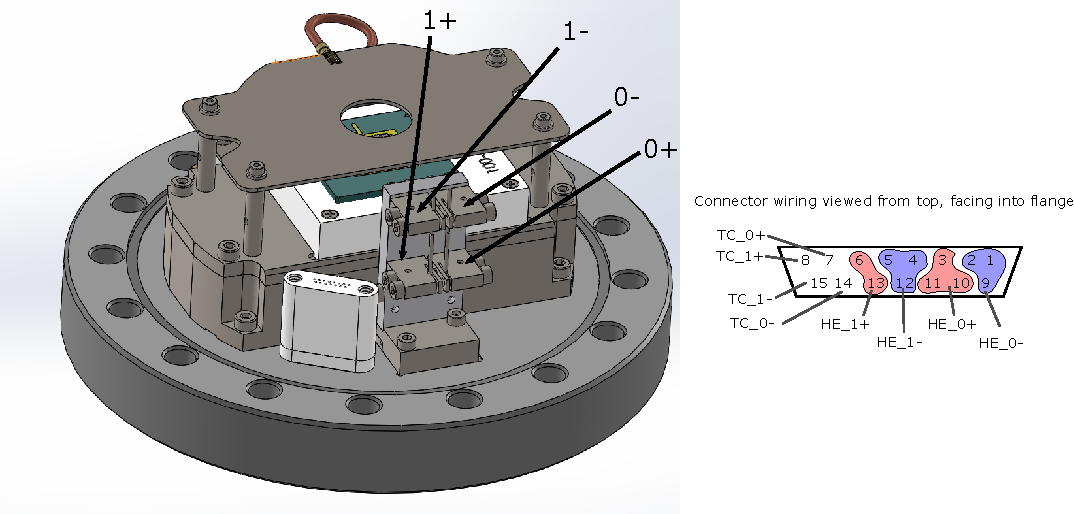
\includegraphics[scale=1]{figures/baseflange_wiring.pdf}
    \caption{Wiring of in vacuum oven connector}
    \label{fig:baseflange_wiring}
\end{figure}

\section{Firmware settings}
All firmware settings are stored within the firmware after writing them in from a configuration file.
An example configuration file can be found in \refsettings{} - some parameters are annotated in that file, others are explained below.
These values are what we have used without issues for a year in two systems, each with two ovens.
To write settings to firmware, you must use \texttt{settings/write.py}, supplying the configuration file as a command line argument.
The programmed settings can be read back using \texttt{settings/read.py}.

\section{Temperature readout}
Run the script \texttt{print\_temperature.py} to print out temperature measurements from both channels in real time. Touch the thermocouples on each tube (with e.g. clean metal tweezers) one after the other to check that the temperature reading changes.

\clearpage
\section{Low power testing}
Measure the current, voltage, and temperature characteristics of the oven at a low/safe power.
Run the script \texttt{low\_power\_heating/measure.py} and enter the channel of oven to be tested.
Use \texttt{low\_power\_heating/plot.py} to make the graph, and the output should look like figure \ref{fig:low_power_heating}.
This measurement determines that everything is connected correctly, the resistance of the oven and wiring, and the polarity of the thermocouple connection.

\begin{figure}
    \center
    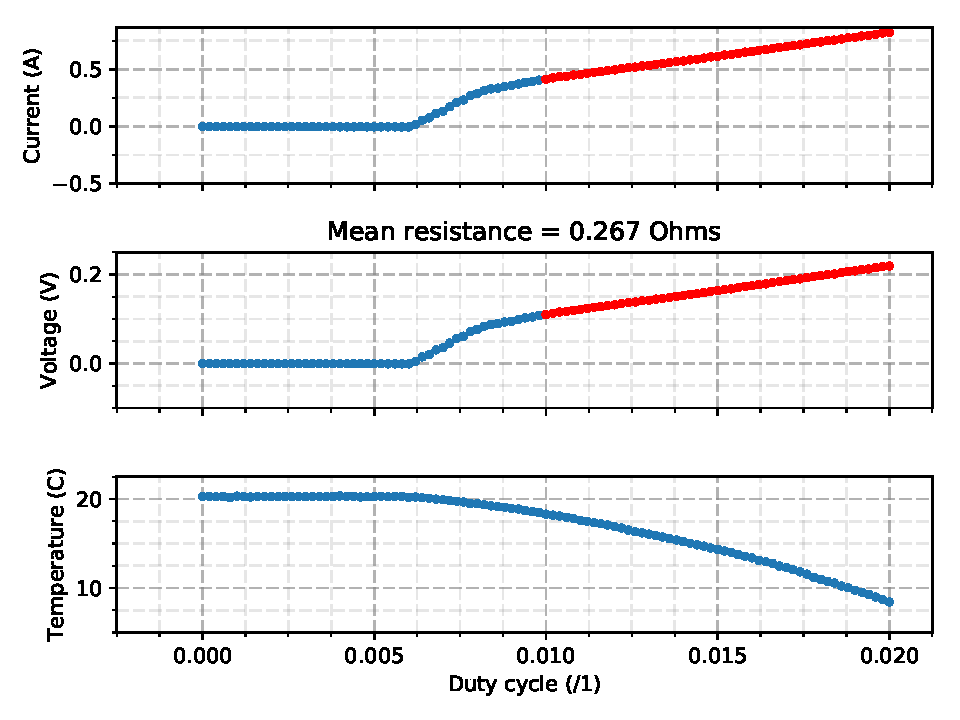
\includegraphics[scale=1]{figures/current_vs_duty_0.pdf}
    \caption{Example data for low\_power\_heating test. NB if the temperature reading decreases throughout the measurement, this indicates that the sensor polarity is inverted}
    \label{fig:low_power_heating}
\end{figure}

In the settings file, the \texttt{cals:<channel>:temperature\_scale} value should be negative if the polarity is inverted.
The numeric value listed in the file is a linearisation around room temperature.

\clearpage
\section{Duty impulse response}

This measurement allows us to determine the temperature-current (T-C) cross-coupling of the oven.
This effect occurs when oven current flows through the thermocouple wiring in the vicinity of the spot weld, which can be mitigated with the weld configuration shown in figure \ref{fig:weld_layout}.
Figures \ref{fig:duty_impulse_response_low} and \ref{fig:duty_impulse_response_high} show this measurement when there is a low and high T-C coefficient respectively.

\begin{figure}
    \center
    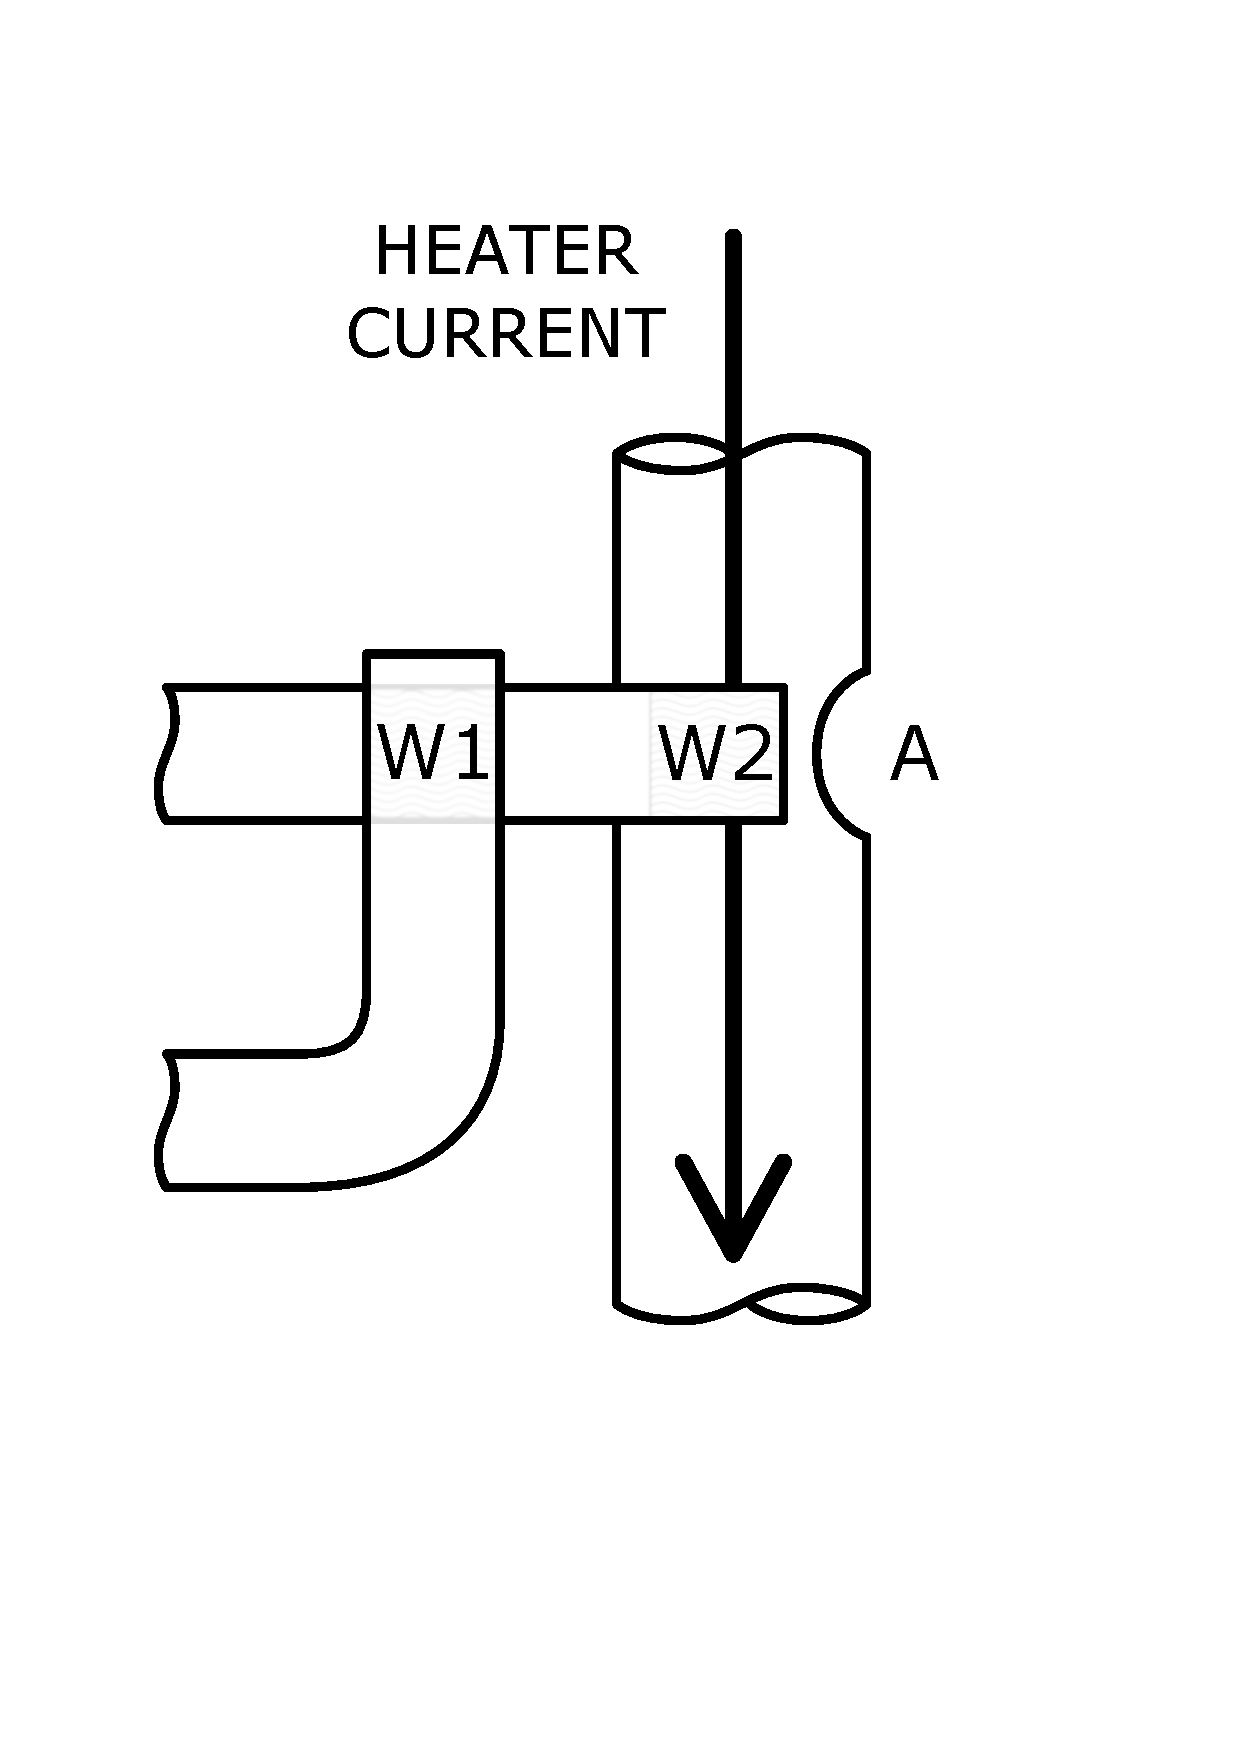
\includegraphics[scale=0.4]{figures/weld_layout.pdf}
    \caption{The thermocouple wires are spot welded to each other at junction W1.
    If the spot weld to the oven tube(W2) is located outside the oven circuit as shown, then no ohmic current flows through the thermocouple circuit and minimal temperature-current cross-coupling occurs.}
    \label{fig:weld_layout}
\end{figure}

\begin{figure}
    \center
    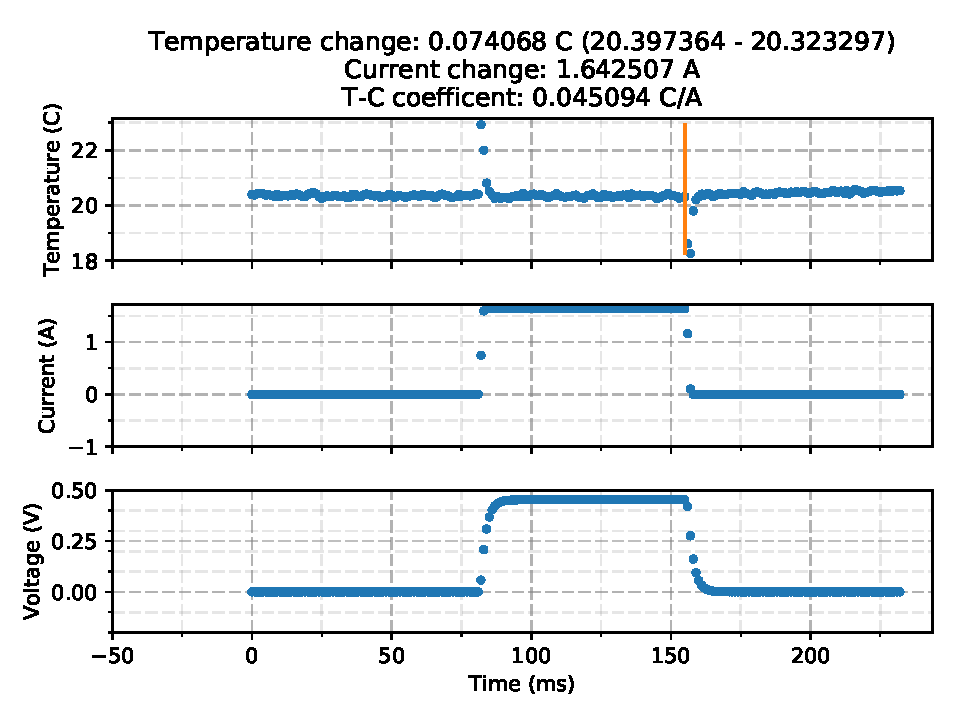
\includegraphics[scale=1]{figures/duty_impulse_response_data_0.pdf}
    \caption{Example data for "duty impulse response" test where there is a low T-C coefficient.}
    \label{fig:duty_impulse_response_low}
\end{figure}

\begin{figure}
    \center
    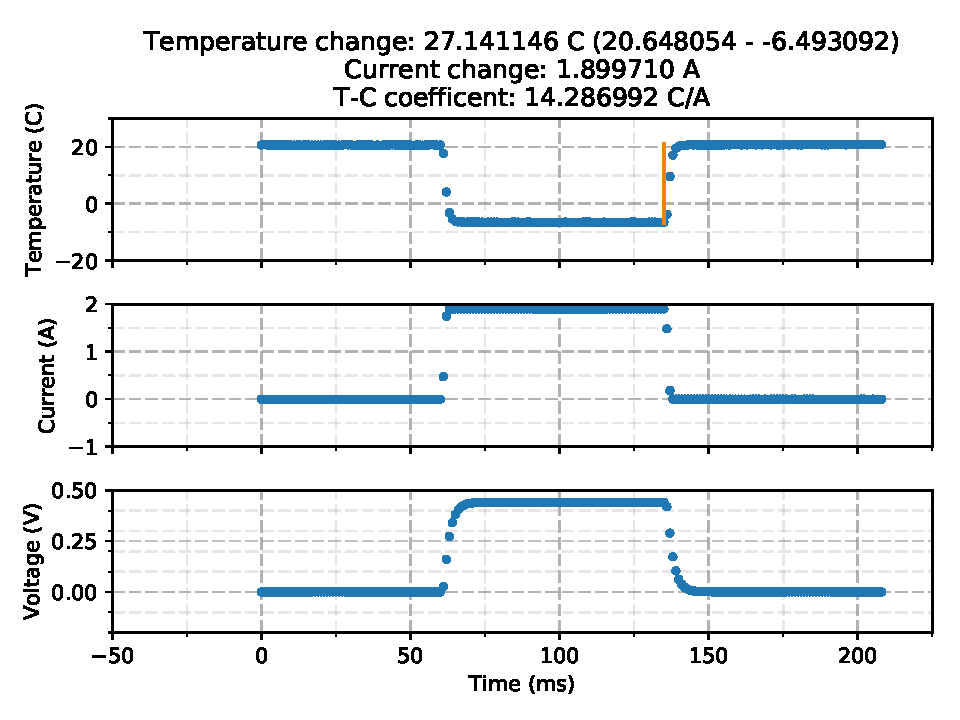
\includegraphics[scale=1]{figures/duty_impulse_response_data_1.pdf}
    \caption{Example data for "duty impulse response" test where there is a high T-C coefficient.}
    \label{fig:duty_impulse_response_high}
\end{figure}

This value is set from \texttt{cals:<channel>:temperature\_current\_coefficient} value in the settings file.

\clearpage
\section{Setup current feedback}

Now the current feedback coefficients need to be set for each channel.
The current feedback controller is a PID controller taking a setpoint in Amps and controlling the duty cycle between 0 and 1.

There are four key parameters for this:
\begin{enumerate}
\item P gain,
\item I gain,
\item D gain,
\item Sample decimation\footnote{Sample decimation is the number of samples to skip before applying feedback. The ADC sampling frequency is \SI{1}{kHz}, so a decimation of 0 will lead to \SI{1}{kHz} update rate, whereas decimation of 4 will lead to one sample every 5 ADC samples giving \SI{200}{Hz}. This is useful when the feedback controller needs to act on long timescales compared with the ADC sampling rate}.
\end{enumerate}
These can be adjusted to optimise the performance of the controller, however I have found the following configuration to work in all cases:
0.008, 0.007, 0, 0.

The script \texttt{setup\_current\_feedback/measure.py} will test the current feedback on the given channel.
The feedback controller parameters are set within the script to the values above.
The output of this script will result in a plot like the one shown in figure \ref{fig:current_feedback}, which allows us to verify that the feedback controller is working correctly (i.e. no oscillation, reasonable response time).

\begin{figure}
    \center
    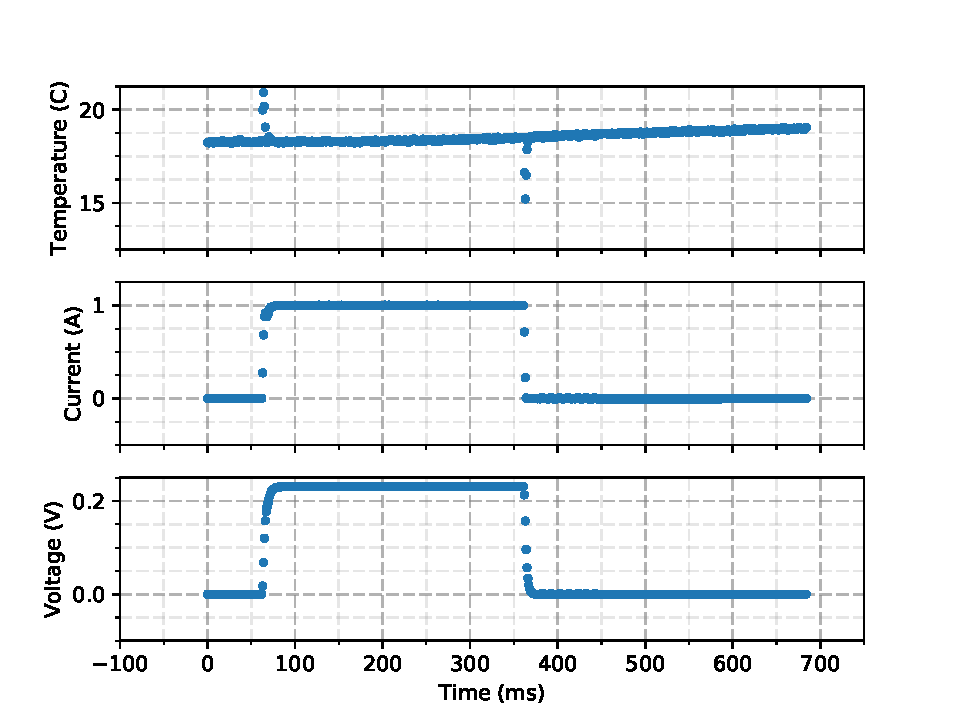
\includegraphics[scale=1]{figures/current_feedback_risetime_data_1.pdf}
    \caption{Example data for setting up the current controller parameters.}
    \label{fig:current_feedback}
\end{figure}

Once satisfied with the current feedback parameters (changing the values hardcoded within the script to try different settings if desired), you can edit the values in the \texttt{configs:current\_<channel>} field of the settings file.

\clearpage
\section{Setup temperature feedback}

Setting of the temperature feedback coefficients is exactly analogous to that of the current feedback.
Use \texttt{setup\_temperature\_feedback/measure.py} to measure the temperature characteristics.
We have found 0.08, 0.008, -0.1 and 9 to work well for the P, I, D gains and sample decimation respectively.


\end{document}
